\begin{figure*}[h!]
    \centering
    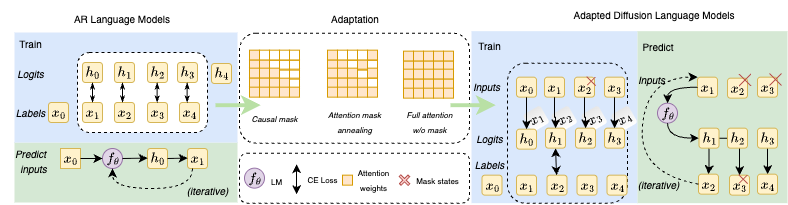
\includegraphics[width=0.95\textwidth]{figs/Adaptation/adaptation.png}
    \caption[Adaptation of AR models to diffusion models]{%
        The overview of Gong et al.'s~\cite{gong_scaling_2025} approach to adapt autoregressive (AR) models to diffusion models. 
        \textbf{Left}: The shift operation in AR models enables the output layer $h_i$ to approximate the distribution of next tokens $x_{i+1}$ in hidden representations through the cross entropy (CE) loss. 
        \textbf{Middle}: Gradually removing the causal mask during training eventually makes the model bidirectional. 
        \textbf{Right}: Inside the diffusion models, shifting the logits to compute the loss with the next token (i.e., the loss on $h_i$ would be concerning $x_{i+1}$), while perceptually, the diffusion models are still functioning as recovering the original signals (since $h_i$ corresponds to $x_{i+1}$ in AR loss).%
    }
    \label{fig:adaptation_overview}
\end{figure*}